\documentclass[12pt, twoside]{article}
\usepackage[francais]{babel}
\usepackage[T1]{fontenc}
\usepackage[latin1]{inputenc}
\usepackage[left=7mm, right=7mm, top=7mm, bottom=7mm]{geometry}
\usepackage{float}
\usepackage{graphicx}
\usepackage{array}
\usepackage{multirow}
\usepackage{amsmath,amssymb,mathrsfs} 
\usepackage{soul}
\usepackage{textcomp}
\usepackage{eurosym}
 \usepackage{variations}
\usepackage{tabvar} 

\begin{document}



\ul{Exercice 1}: Calculer les expressions suivantes. 

\enskip


$A=\dfrac{7}{12}+\dfrac{1}{2}$; \qquad  \qquad
\qquad $B=\dfrac{7}{16}-\dfrac{3}{4}$; \qquad \qquad \qquad
$C=\dfrac{3}{20}-\dfrac{9}{5}$; \qquad \qquad
\qquad $D=\dfrac{4}{9}+\dfrac{7}{54}$.



\bigskip


\ul{Exercice 2}: Calculer les expressions suivantes et donner le r�sultat sous
la forme d'une fraction irr�ductible.

\enskip

$E=\dfrac{3}{8}-\dfrac{4}{5}$; \qquad  $F=\dfrac{-6}{13}+\dfrac{1}{4}$;
\qquad  $G=\dfrac{6}{7}-\dfrac{1}{3}$;  \qquad
$H=\dfrac{2}{11}+\dfrac{-3}{5}$;\qquad
$I=\dfrac{5}{6}+\dfrac{-4}{3}-\dfrac{3}{2}$; \qquad
$J=\dfrac{3}{7}-\dfrac{5}{14}+\dfrac{7}{2}$.


\bigskip

\ul{Exercice 3}: Calculer $M=\dfrac{x}{12}+\dfrac{y}{8}$ pour $x=1$ et $y=-2$.


\bigskip


\ul{Exercice 4}: Ecrire les inverses de chacun des nombres suivants:

\enskip

$\dfrac{3}{2}$; \qquad \qquad $\dfrac{-2}{5}$; \qquad \qquad $\dfrac{1}{4}$;
\qquad \qquad $\dfrac{-1}{4}$;\qquad \qquad $4$; \qquad \qquad $1$;\qquad \qquad
$-1$.

\bigskip

\ul{Exercice 5}: Compl�ter si possible par un nombre en �criture fractionnaire:

$\dfrac{2}{3} \times \ldots \ldots =1$ \qquad \qquad \qquad
\qquad $\dfrac{-5}{6} \times \ldots \ldots =1$ \qquad \qquad \qquad
\qquad $\dfrac{0,3}{-4} \times \ldots \ldots =1$ 


$(-\dfrac{5}{7})
\times \ldots \ldots =1$ \qquad \qquad \qquad \qquad $\dfrac{-5}{-4} \times
\ldots \ldots =1$ \qquad \qquad \qquad \qquad $\dfrac{0}{2} \times \ldots \ldots
=1$

\bigskip


\ul{Exercice 6}: Calcul mental!

Sachant que $\dfrac{1}{5}=0,2$; calculer $\dfrac{2}{5}$; \quad $\dfrac{11}{5}$;
\quad $-\dfrac{7}{5}$; \quad $-\dfrac{8}{5}$.



\bigskip

\bigskip


\ul{Exercice 1}: Calculer les expressions suivantes. 

\enskip


$A=\dfrac{7}{12}+\dfrac{1}{2}$; \qquad  \qquad
\qquad $B=\dfrac{7}{16}-\dfrac{3}{4}$; \qquad \qquad \qquad
$C=\dfrac{3}{20}-\dfrac{9}{5}$; \qquad \qquad
\qquad $D=\dfrac{4}{9}+\dfrac{7}{54}$.



\bigskip


\ul{Exercice 2}: Calculer les expressions suivantes et donner le r�sultat sous
la forme d'une fraction irr�ductible.

\enskip

$E=\dfrac{3}{8}-\dfrac{4}{5}$; \qquad  $F=\dfrac{-6}{13}+\dfrac{1}{4}$;
\qquad  $G=\dfrac{6}{7}-\dfrac{1}{3}$;  \qquad
$H=\dfrac{2}{11}+\dfrac{-3}{5}$;\qquad
$I=\dfrac{5}{6}+\dfrac{-4}{3}-\dfrac{3}{2}$; \qquad
$J=\dfrac{3}{7}-\dfrac{5}{14}+\dfrac{7}{2}$.


\bigskip

\ul{Exercice 3}: Calculer $M=\dfrac{x}{12}+\dfrac{y}{8}$ pour $x=1$ et $y=-2$.


\bigskip


\ul{Exercice 4}: Ecrire les inverses de chacun des nombres suivants:

\enskip

$\dfrac{3}{2}$; \qquad \qquad $\dfrac{-2}{5}$; \qquad \qquad $\dfrac{1}{4}$;
\qquad \qquad $\dfrac{-1}{4}$;\qquad \qquad $4$; \qquad \qquad $1$;\qquad \qquad
$-1$.

\bigskip

\ul{Exercice 5}: Compl�ter si possible par un nombre en �criture fractionnaire:

$\dfrac{2}{3} \times \ldots \ldots =1$ \qquad \qquad \qquad
\qquad $\dfrac{-5}{6} \times \ldots \ldots =1$ \qquad \qquad \qquad
\qquad $\dfrac{0,3}{-4} \times \ldots \ldots =1$ 


$(-\dfrac{5}{7})
\times \ldots \ldots =1$ \qquad \qquad \qquad \qquad $\dfrac{-5}{-4} \times
\ldots \ldots =1$ \qquad \qquad \qquad \qquad $\dfrac{0}{2} \times \ldots \ldots
=1$

\bigskip


\ul{Exercice 6}: Calcul mental!

Sachant que $\dfrac{1}{5}=0,2$; calculer $\dfrac{2}{5}$; \quad $\dfrac{11}{5}$;
\quad $-\dfrac{7}{5}$; \quad $-\dfrac{8}{5}$.
\pagebreak


\begin{tabular}{cc}
\begin{minipage}{9cm}

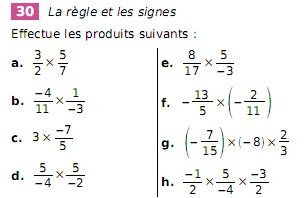
\includegraphics[width=9cm]{images/ex30p36.jpg}

\bigskip

\bigskip


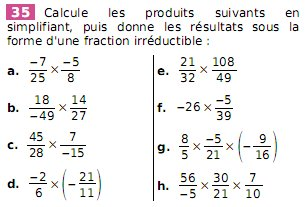
\includegraphics[width=9cm]{images/ex35p36.jpg}

\bigskip

\bigskip

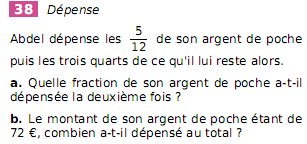
\includegraphics[width=9cm]{images/ex38p36.jpg}






\end{minipage}
&
\begin{minipage}{9cm}

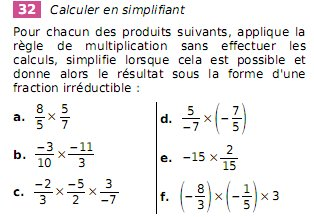
\includegraphics[width=9cm]{images/ex32p36.jpg}

\bigskip

\bigskip

\bigskip

\bigskip

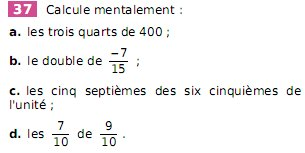
\includegraphics[width=9cm]{images/ex37p36.jpg}




\bigskip

\bigskip

\bigskip

\bigskip

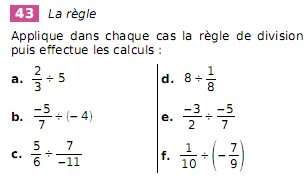
\includegraphics[width=9cm]{images/ex43p37.jpg}






\end{minipage}
\end{tabular}


\pagebreak

\begin{tabular}{cc}
\begin{minipage}{9cm}



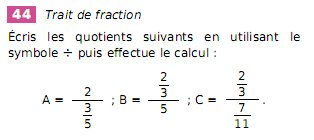
\includegraphics[width=9cm]{images/ex44p37.jpg}

\bigskip

\bigskip

\bigskip

\bigskip

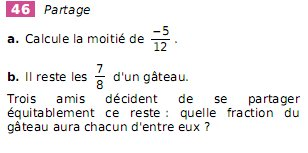
\includegraphics[width=9cm]{images/ex46p37.jpg}

\bigskip

\bigskip

\bigskip

\bigskip

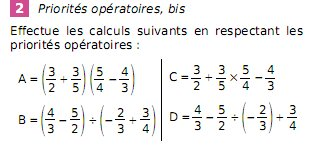
\includegraphics[width=9cm]{images/ex49p38.jpg}


\end{minipage}
&
\begin{minipage}{9cm}




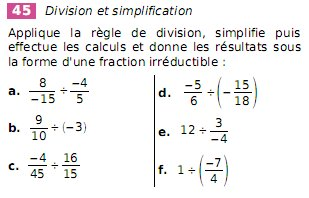
\includegraphics[width=9cm]{images/ex45p37.jpg}

\bigskip

\bigskip

\bigskip

\bigskip

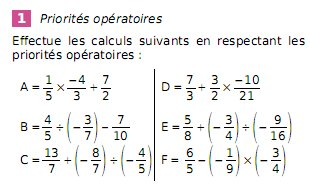
\includegraphics[width=9cm]{images/ex48p38.jpg}


\bigskip

\bigskip

\bigskip

\bigskip


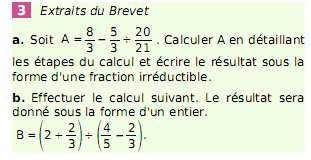
\includegraphics[width=9cm]{images/ex50p38.jpg}

\end{minipage}
\end{tabular}

\end{document}
